\documentclass[../main.tex]{subfiles}
\begin{document}

%----------------------------
%		Task 1.1
%----------------------------
\subsection{What is the core idea of deep learning? How does it differ from shallow learning?}

The core idea of deep learning is to have several hidden layers to describe complicated functions. This enables more complex representations, with the disadvantage of more computing power needed, as well as overfitting. \autoref{fig:deep_example} shows a diagram of a deep neural network, where $\mathbf{u}=\{u_1, u_2\}$, $\mathbf{v}=\{v_1, v_2\}$, and the cloud denotes hidden layers. 

A shallow network contains fewer, if any, hidden layers. It can represent all functions, but the number of parameters expands rapidly with the complexity of the function. It is less prone to overfitting. A shallow network is displayed in \autoref{fig:shallow_example}, where $\mathbf{u}=\{u_1, u_2\}$ is the only hidden layer.

\begin{figure}
    \centering
    \begin{subfigure}[b]{0.48\textwidth}
    	\centering
        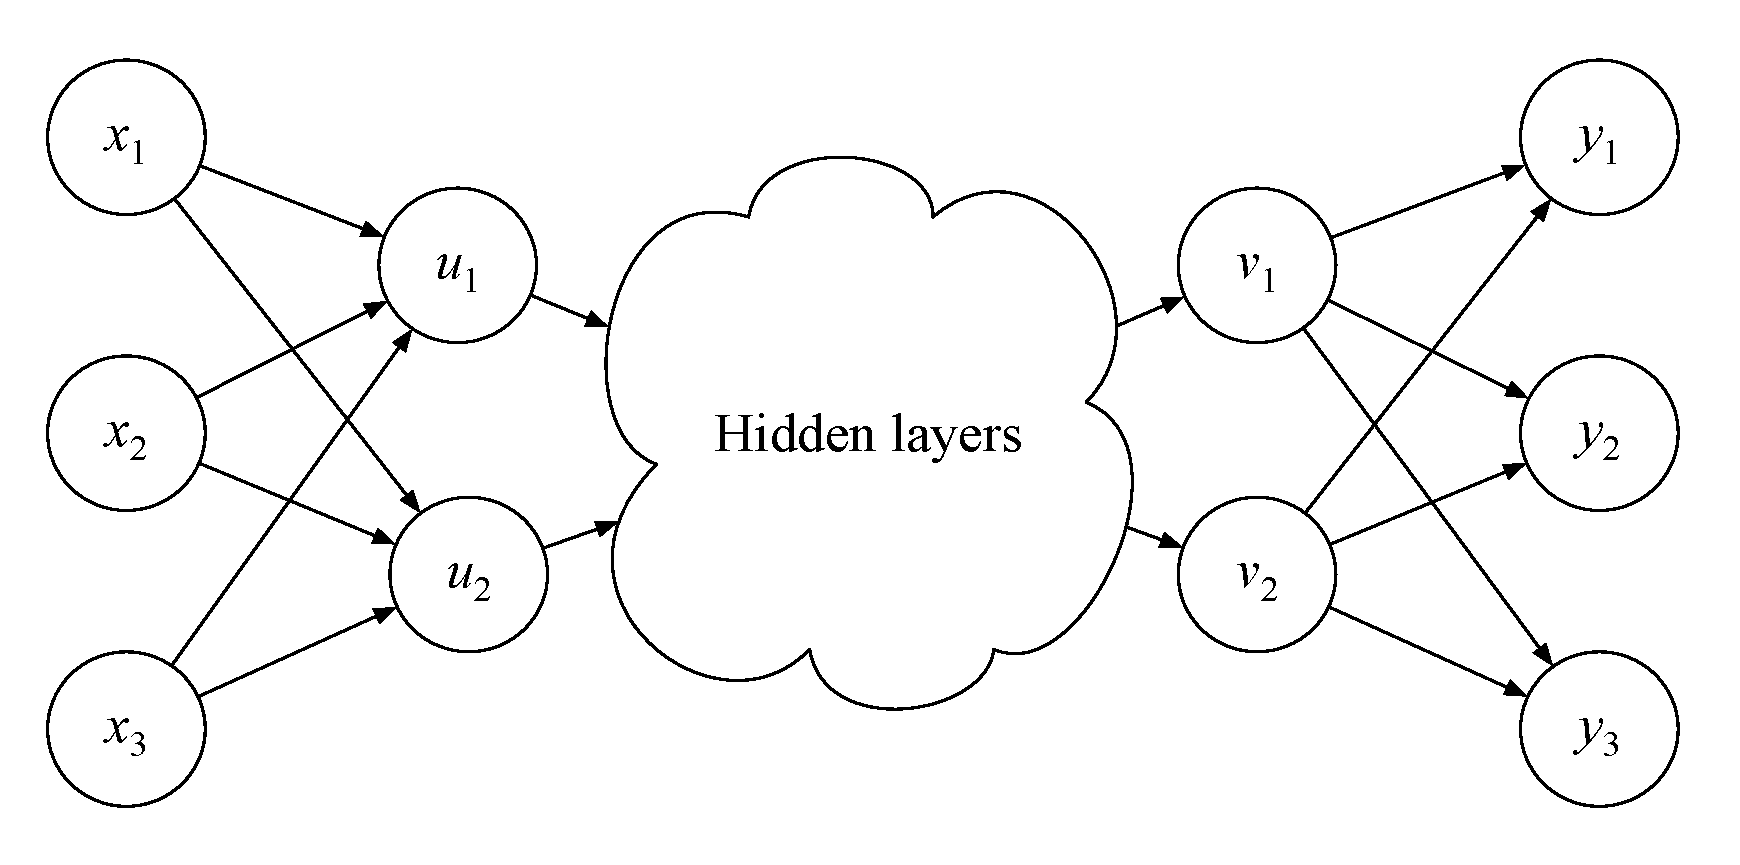
\includegraphics[height=3cm]{figures/theory/deep_network}
        \caption{Example of a deep network}
        \label{fig:deep_example}
    \end{subfigure}
    ~
    \begin{subfigure}[b]{0.48\textwidth}
    	\centering
        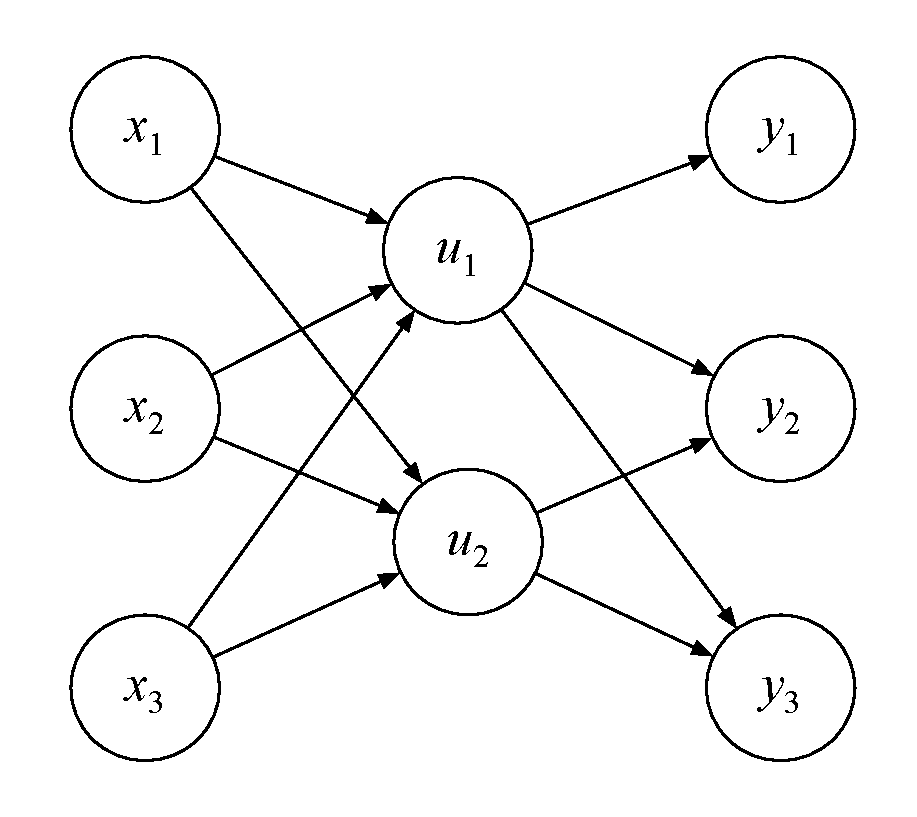
\includegraphics[height=3cm]{figures/theory/shallow_network}
        \caption{Example of a shallow network}
        \label{fig:shallow_example}
    \end{subfigure}
    \caption{Deep and shallow networks.}\label{fig:deep_shallow}
\end{figure}

%----------------------------
%		Task 1.2
%----------------------------
\subsection{Logistic regression as neural network}
One can define the logistic regression implemented in Assignment 1 \cite{assignment1} as a neural network, where we have one hidden layer with one neuron. One first define the input to the neuron as
\begin{equation}
	z = h(\mbf{x}) =\mbf{w}^{\rm T} \mbf{x} \label{eq:z}
\end{equation}
The activation function is then defined as
\begin{equation}
	\sigma(z)=\frac{1}{1+e^{-z}}
\end{equation}
and the backpropagation algorithm is then
\begin{equation}
	\frac{\partial E_{\rm ec}(\mathbf{w})}{\partial \mathbf{w}} = 
		\frac{\partial E_{\rm ec}(\mathbf{w})}{\partial \sigma(z)}
		\cdot \frac{\partial \sigma(z)}{\partial z}
		\cdot \frac{\partial z}{\partial \mathbf{w}}.
\end{equation}
The training will then be
\begin{equation}
	\mbf{w}(k+1) \leftarrow \mbf{w}(k) - \eta \sum_{i=1}^{N}(\sigma(z)-y_i)\mbf{x}_i
\end{equation}
The final parameter is given by
\begin{equation}
	y_1 = \sigma(z).
\end{equation}
The topology of the network is shown in \autoref{fig:log_example}.

\begin{figure}
	\centering
    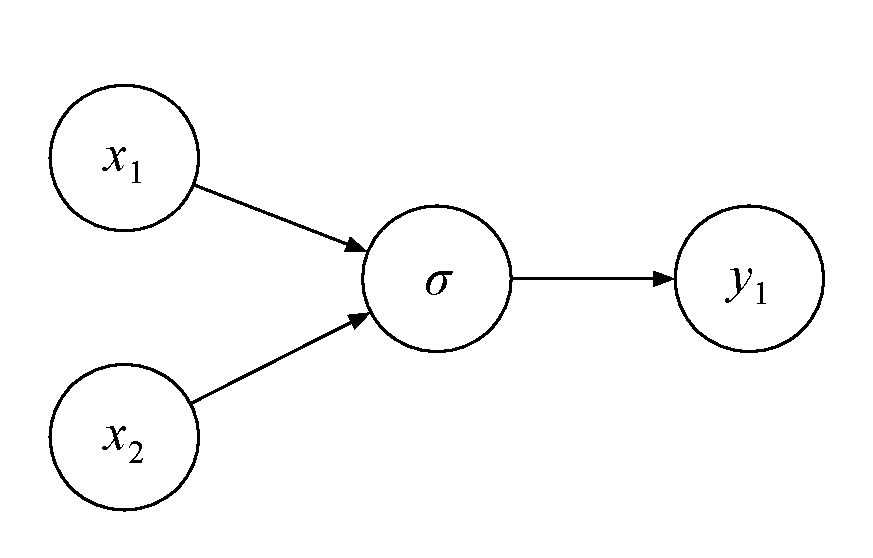
\includegraphics[height=3cm]{figures/theory/log_network}
    \caption{Example of a logistic regression neural network}
    \label{fig:log_example}
\end{figure}

%----------------------------
%		Task 1.3
%----------------------------
\subsection{Artificial neural network with only linear activation functions}

Lets assume we have a linear activation function on the form
\begin{equation}
	a(z) = C_1 \cdot z + C_2
\end{equation}
where $C_1$ and $C_2$ are constant. Traditionally, the backprogation algorithm would be defined as
\begin{equation}
	\frac{\partial E}{\partial w_j} = 
	\frac{\partial E}{\partial a(z_j)}
	\cdot\frac{\partial a(z_j)}{\partial z_j}
	\cdot\frac{\partial z_j}{\partial w_j}
\end{equation}
where
\begin{equation}
	E=\frac{1}{2}\sum_{j}(y_j-a_j)
\end{equation}
and $z_j$ is defined by \autoref{eq:z}. The first differential is then given by
\begin{equation}
	\frac{\partial E}{\partial a(z_j)} = -(y_j-a_j)
\end{equation}
The second differential will be constant, as
\begin{equation}
	\frac{\partial a(z_j)}{\partial z_j} = \frac{\partial}{\partial z_j} \big( C_1 \cdot z + C_2 \big) = C_1
\end{equation}
The last differential is then
\begin{equation}
	\frac{\partial z_j}{\partial w_j} = \frac{\partial}{\partial w_j}\big( w_j \cdot x_j \big) = x_j
\end{equation}
This gives a backpropagation algorithm on the form
\begin{equation}
	\frac{\partial E}{\partial w_j} = -C_1x_j(y_j-a_j) =  \big(C_1^2 x_j^2\big) w_j - \big(C_1x_jy_j+C_1C_2x_j)
\end{equation}
where $C_1^2 x_j^2$ and $- \big(C_1x_jy_j+C_1C_2x_j)$ are constant with respect to $w_j$, so that
\begin{equation}
	\frac{\partial E}{\partial w_j} = K_1 w_j + K_2
\end{equation}
Aforementioned implies that any transition through any node will be linear. A cascade of linear operations always results in a linear system, leading to the transfer function of the neural network to be linear as well.

%----------------------------
%		Task 1.3
%----------------------------
\subsection{Forward Pass for Network Topology}

The first layer $\mbf{u}$ is given by
\begin{equation}
	\mbf{u} = \sigma(\mbf{W}^{(1)\rm T} \mbf{x}) = \vari{x_1}
\end{equation}
and the second layer will be
\begin{equation}
	\mbf{v} = \sigma( \mbf{W}^{(2)\rm T} \mbf{u}) =\vari{x_2}
\end{equation}
resulting in the output value
\begin{equation}
	\mbf{y}=\mbf{W}^{(3)\rm T}\sigma(\mbf{v}) = \vari{x_3}
\end{equation}
The values have been calculated using an attached python module.


\end{document}